\begin{enumerate}
	\item[(a)] Show that the pendulum model has index 3.
	\begin{align*}
		m\,\ddot x &= x\,\lambda\\
		m\,\ddot y &= y\,\lambda - m\,g\\
		0 &= x^2 + y^2 - l^2		
	\end{align*}
	Let, 
	\begin{align*}
		\dot x &= u & e_1\\
		\dot y &= v & e_2\\
		m\,\dot u &= x\,\lambda & e_3\\
		m\,\dot v &= y\,\lambda - m\,g & e_4\\
		0 &= x^2 + y^2 - l^2 & e_5
	\end{align*}
	From the physics, the states are $x,\,y,\,u,\,v,\,\lambda$. We need to get $\dot\lambda$ to reduce the DAE to an ODE equation set. Therefore, we differentiate $e_3$ 3 times. Then we get:
	\begin{align*}
		\dot x &= u & e_1\\
		\dot y &= v & e_2\\
		m\,\dot u &= x\,\lambda & e_3\\
		m\,\dot v &= y\,\lambda - m\,g & e_4\\
		\dot \lambda &= -3\,\frac{v}{l^2}\,m\,g &  \dddot e_5
	\end{align*}
	\fbox{\begin{minipage}[h!]{\textwidth}
			Therefore, the differential index is 3.
	\end{minipage}}	
	\item[(b)] Perform index reduction by differentiating model equations.
	The model is given as follows:
	\begin{align*}
		\dot x &= u & e_1\\
		\dot y &= v & e_2\\
		m\,\dot u &= x\,\lambda & e_3\\
		m\,\dot v &= y\,\lambda - m\,g & e_4\\
		0 &= x^2 + y^2 - l^2 & e_5
	\end{align*}
	Differentiating $e_5$ two times we reduce the system to a DAE with index 1. i.e:
	\begin{align*}
		\dot x &= u & e_1\\
		\dot y &= v & e_2\\
		m\,\dot u &= x\,\lambda & e_3\\
		m\,\dot v &= y\,\lambda - m\,g & e_4\\
		0 &= u^2 + v^2 +\lambda\,\frac{x^2 + y^2}{m} - g\,y & \ddot e_5
	\end{align*}
	Simulating the DAE using Matlab gives the following:

	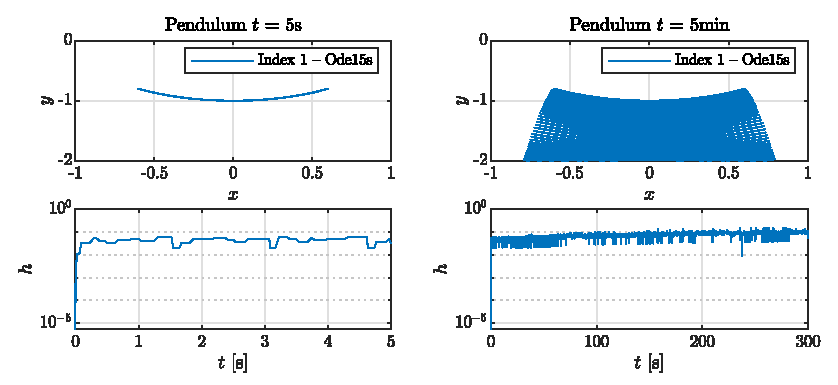
\includegraphics[width=\textwidth]{Figures/Ugf2_14a.eps}
	
	From the above figure it is clear that for a longer simulation time the algebraic constraint given by $e_5$ is no longer satisfied. 
	
	\item[(c)] Better index reduction using  baumgartner stabilization.
	Here, $\ddot e_5$ is replaced with $\ddot e_5 + \alpha\,\dot e_5 + \beta\,e_5$, and $\alpha$, $\beta$ are chosen such that the zeros of $s^2 + \alpha\,s + \beta = 0 $ are to the left half of the $s$-plane. 
	
	For the simulation using  baumgartner stabilization, $\alpha = \beta = 1$. The following figures presents the simulation results:
	
	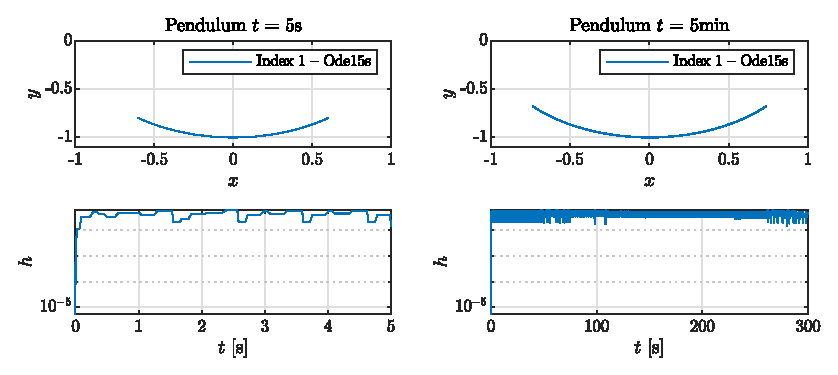
\includegraphics[width=0.9\textwidth]{Figures/Ugf2_14c.eps}
	
	\item[(d)] Add $\epsilon\,\dot \lambda$ on the left-hand-side of the algebraic constraints and simulate using an ODE solver.
	In the model described previously, $e_5$ not becomes as follows:
	\begin{align*}
		\epsilon\,\dot \lambda &= u^2 + v^2 +\lambda\,\frac{x^2 + y^2}{m} - g\,y & \ddot e_5
	\end{align*}
	The matlab solver \texttt{ode45} is unable to meet integration tolerances without reducing the step size below the smallest value allowed (5.551115e-17). The case with $\epsilon=0$ was simulated using \texttt{ode15s}.
	
	Here is the simulation results:
	
	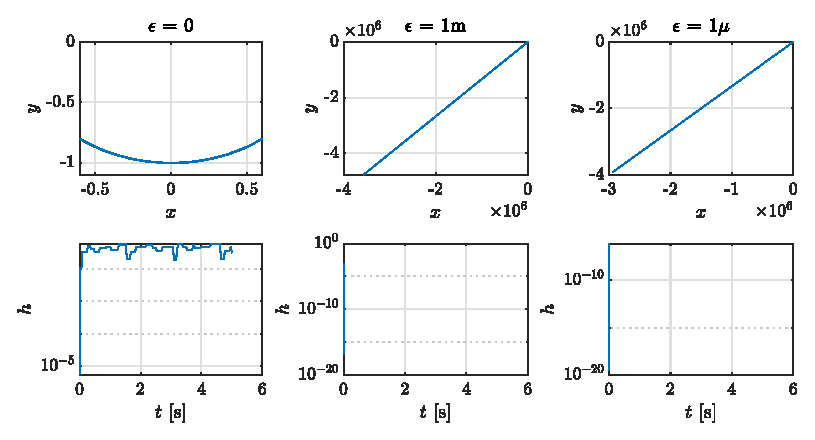
\includegraphics[width=0.55\textheight]{Figures/Ugf2_14d.eps}
	
	Here is the code:
	
	\begin{lstlisting}
		epsilon = [0 1e-3 1e-6]; 
		
		% function definition
		% in pendulam_idx1 y(1) = x, y(2) = y, y(3) = u, y(4) = v, y(5) = lambda
		% lambda from algebraic constraint
		pendulam_idx1_zz = @(t,y) [y(3); y(4); y(5)*y(1); y(5)*y(2) - m*g;
		y(3)^2 + y(4)^2 + y(5)*(y(1)^2 + y(2)^2)/m - g*y(2)]; 
		% Direct index reduction technique
		
		M_idx1_zz = [1 0 0 0 0;
		0 1 0 0 0;
		0 0 m 0 0;
		0 0 0 m 0;
		0 0 0 0 0]; % Mass matrix
		
		M_idx1_zz(end) = epsilon(1);
		options_idx1_zz = odeset('Mass',M_idx1_zz); 
		[t_idx1_l_zz_1,y_idx1_l_zz_1] = ode15s(@(t,y) pendulam_idx1_zz(t,y),tsim_s,y0_idx1,options_idx1_zz);
		
		M_idx1_zz(end) = epsilon(2);
		options_idx1_zz = odeset('Mass',M_idx1_zz); 
		[t_idx1_l_zz_2,y_idx1_l_zz_2] = ode45(@(t,y) pendulam_idx1_zz(t,y),tsim_s,y0_idx1,options_idx1_zz);
		
		M_idx1_zz(end) = epsilon(3);
		options_idx1_zz = odeset('Mass',M_idx1_zz); 
		[t_idx1_l_zz_3,y_idx1_l_zz_3] = ode45(@(t,y) pendulam_idx1_zz(t,y),tsim_s,y0_idx1,options_idx1_zz);
	\end{lstlisting}
\end{enumerate}